%# -*- coding: utf-8-unix -*-
%%==================================================
\chapter{计算机视觉CV}\label{AIChapter11}
%%%%%%%%%%%%%%%%%%%%%%%%%%%%%%%%%%%%%%%%%%
\begin{figure}[H]
\centering
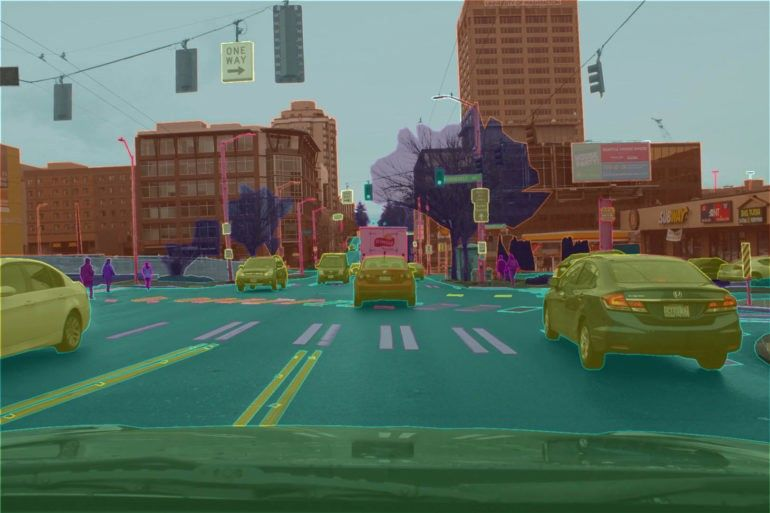
\includegraphics[width=0.76\textwidth]{CV20191218130058.jpg}
\label{CV20191218130058}
\end{figure}
%%%%%%%%%%%%%%%%%%%%%%%%%%%%%%%%%%%%%%%%%%
%\begin{figure}[htbp]
%	\centering
%	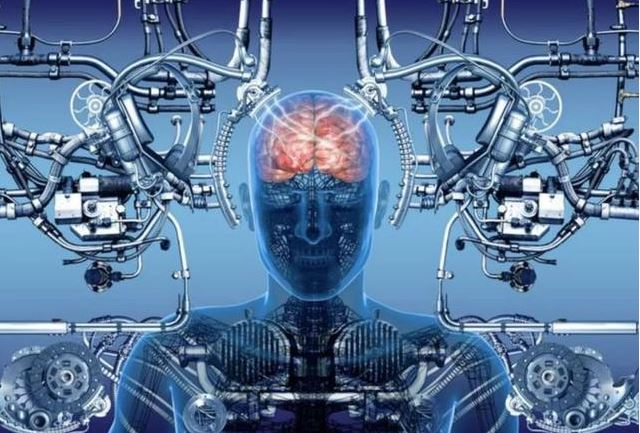
\includegraphics[width=0.75\textwidth]{AI20191217151400.jpg}
%   \label{AI:turingFig0000001}
%\end{figure} 深度学习扩展了数字图像处理的边界。然而, 这并不代表在深度学习崛起之前不断发展进步的传统计算机视觉技术被淘汰。近期, 来自爱尔兰垂利理工学院的研究者发表论文, 分析了这两种方法的优缺点。
%%%%%%%%%%%%%%%%%%%%%%%%%%%%%%%%%%%%%%%%%%
\newpage
\section{深度学习 VS 传统计算机视觉}
Deep Learning vs. Traditional Computer Vision, CVC 2019  Apr 25, 2019 - Apr 26, 2019. Las Vegas, Nevada, United States \cite{MahonyCVC2019}

Animal Face、Anime Face、Oxford Flower、CUB-200-2011和Caltech-256数据集


\subsection{深度学习的优势}

深度学习的快速发展和设备能力的改善(如算力、内存容量、能耗、图像传感器分辨率和光学器件)提升了视觉应用的性能和成本效益, 并进一步加快了此类应用的扩展。与传统 CV 技术相比, 深度学习可以帮助 CV 工程师在图像分类、语义分割、目标检测和同步定位与地图构建(SLAM)等任务上获得更高的准确率。由于深度学习所用的神经网络是训练得到而非编程得到, 因此使用该方法的应用所需的专家分析和微调较少, 且能够处理目前系统中的海量可用视频数据。深度学习还具备绝佳的灵活性, 因为对于任意用例, CNN 模型和框架均可使用自定义数据集重新训练, 这与 CV 算法不同, 后者具备更强的领域特定性。

以移动机器人的目标检测问题为例, 对比这两类计算机视觉算法:

传统计算机视觉方法使用成熟的 CV 技术处理目标检测问题, 如特征描述子(SIFT、SUR、BRIEF 等)。在深度学习兴起前, 图像分类等任务需要用到特征提取步骤, 特征即图像中「有趣」、描述性或信息性的小图像块。这一步可能涉及多种 CV 算法, 如边缘检测、角点检测或阈值分割算法。从图像中提取出足够多的特征后, 这些特征可形成每个目标类别的定义(即「词袋」)。部署阶段中, 在其他图像中搜索这些定义。如果在一张图像中找到了另一张图像词袋中的绝大多数特征, 则该图像也包含同样的目标(如椅子、马等)。

传统 CV 方法的缺陷是:从每张图像中选择重要特征是必要步骤。而随着类别数量的增加, 特征提取变得越来越麻烦。要确定哪些特征最能描述不同的目标类别, 取决于 CV 工程师的判断和长期试错。此外, 每个特征定义还需要处理大量参数, 所有参数必须由 CV 工程师进行调整。
深度学习引入了端到端学习的概念, 即向机器提供的图像数据集中的每张图像均已标注目标类别。因而深度学习模型基于给定数据「训练」得到, 其中神经网络发现图像类别中的底层模式, 并自动提取出对于目标类别最具描述性和最显著的特征。人们普遍认为 DNN 的性能大大超过传统算法, 虽然前者在计算要求和训练时间方面有所取舍。随着 CV 领域中最优秀的方法纷纷使用深度学习, CV 工程师的工作流程出现巨大改变, 手动提取特征所需的知识和专业技能被使用深度学习架构进行迭代所需的知识和专业技能取代(见图 1)。
%%%%%%%%%%%%%%%%%%%%%%%%%%%%%%%%%%%%%%%%%%
\begin{figure}[http]
\centering
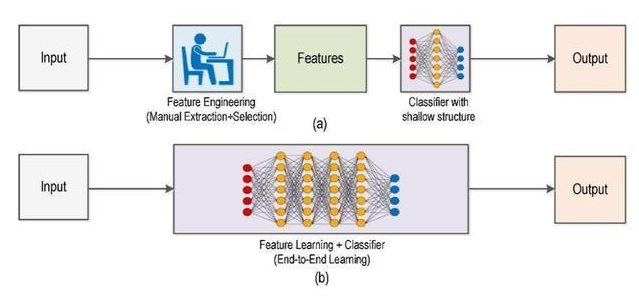
\includegraphics[width=0.86\textwidth]{DPLandCV20191224001.png}
\caption{a)传统计算机视觉工作流 vs b)深度学习工作流\cite{WANG2018144}}
\label{DPLandCV20191224001}
\end{figure}

近年来, CNN 的发展对 CV 领域产生了巨大影响, 也使得目标识别能力出现大幅提升。这种爆发与算力的提升、训练数据量的增加密不可分。近期 CV 领域中深度神经网络架构出现井喷并得到广泛应用, 这从论文《\href{http://papers.nips.cc/paper/4824-imagenet-classification-with-deep-convolutional-neural-networks}{ImageNet Classification with Deep Convolutional Neural Networks}》引用量超 3000 次中可见一斑。

CNN 利用卷积核(又称滤波器)来检测图像中的特征(如边)。卷积核是权重矩阵, 这些权重被训练用于检测特定特征。如名字所示, CNN 的主要思想是在给定输入图像上空间性地卷积内核, 检查是否出现检测所需特征。为了用数值表示出现某个特征的置信度, 神经网络执行卷积操作, 即计算卷积核与它和输入图像重叠区域的点积(卷积核正在查看的原始图像区域叫做感受野)。

为了促进卷积核权重的学习, 研究人员向卷积层的输出添加偏置项, 并馈入非线性激活函数中。激活函数通常是非线性函数, 如 Sigmoid、TanH 和 ReLU。激活函数的选择取决于数据和分类任务的性质。例如, ReLU 具备更多生物表征(大脑中的神经元是否处于激活状态)。因此, 在图像识别任务中, ReLU 会得到更好的结果, 因为它对梯度消失问题具备更强的抵抗力, 而且它能够输出更稀疏、高效的表征。

为了加速训练过程, 减少网络消耗的内存量, 卷积层后通常跟着一个池化层, 用于移除输入特征中的冗余部分。例如, 最大池化在输入上移动窗口, 仅输出窗口中的最大值, 从而高效减少图像中的冗余部分, 留下重要像素。如图 2 所示, 深度 CNN 可能具备多对卷积和池化层。最后, 全连接层将上一层压缩为特征向量, 然后输出层利用密集网络计算输出类别/特征的分数(置信度或概率)。将该输出输入到回归函数中, 如 Softmax 函数, 它将所有事物映射为向量且其中所有元素的总和为 1。
%%%%%%%%%%%%%%%%%%%%%%%%%%%%%%%%%%%%%%%%%%
\begin{figure}[http]
\centering
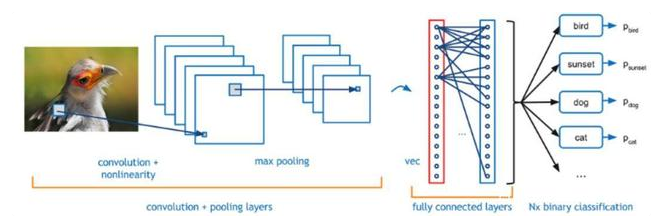
\includegraphics[width=0.86\textwidth]{DPLandCV20191224002.png}
\caption{CNN 构造块。(图源:\href{https://adeshpande3.github.io/adeshpande3.github.io/A-Beginner\%27s-Guide-To-Understanding-Convolutional-Neural-Networks/}{[13]})}
\label{DPLandCV20191224002}
\end{figure}

但是深度学习仍然只是 CV 领域的工具。例如, CV 领域中最常用的神经网络是 CNN。那么什么是卷积呢?卷积广泛应用于图像处理技术。(深度学习的优点很明确, 本文暂不讨论当前最优算法。)但深度学习并非解决所有问题的万灵药, 下文将介绍传统 CV 算法更适合的问题及应用。
%%%%%%%%%%%%%%%%%%%%%%%%%%%%%%%%%%%%%%%%%%
\subsection{传统 CV 技术的优势}

基于特征的传统方法在 CV 任务中能够有效提升性能的原因。这些传统方法包括:
\begin{itemize}
\item 尺度不变特征变换(Scale Invariant Feature Transform, SIFT)[14]
\item 加速稳健特征(Speeded Up Robust Feature, SURF)[15]
\item 基于加速分割测试的特征(Features from Accelerated Segment Test, FAST)\cite{Rosten2006}
\item 霍夫变换(Hough transform)\cite{Goldenshluger2004}
\item 几何哈希(Geometric hashing)[18]
\item 特征描述子(如 SIFT 和 SURF)通常与传统机器学习分类算法(如支持向量机和 K 最近邻算法)结合使用, 来解决 CV 问题。
\end{itemize}

深度学习有时会「过犹不及」, 传统 CV 技术通常能够更高效地解决问题, 所用的代码行数也比深度学习少。SIFT, 甚至简单的色彩阈值和像素计数等算法, 都不是特定于某个类别的, 它们是通用算法, 可对任意图像执行同样的操作。与之相反, 深度神经网络学得的特征是特定于训练数据的。也就是说, 如果训练数据集的构建出现问题, 则网络对训练数据集以外的图像处理效果不好。

因此, SIFT 等算法通常用于图像拼接/3D 网格重建等应用, 这些应用不需要特定类别知识。这些任务也可以通过训练大型数据集来实现, 但是这需要巨大的研究努力, 为一个封闭应用费这么大劲并不实际。在面对一个 CV 应用时, 工程师需要培养选择哪种解决方案的常识。例如, 对流水线传送带上的两类产品进行分类, 一类是红色一类是蓝色。深度神经网络需要首先收集充足的训练数据。然而, 使用简单的色彩阈值方法也能达到同样的效果。一些问题可以使用更简单、快速的技术来解决。
如果 DNN 对训练数据以外的数据效果不好, 怎么办?在训练数据集有限的情况下, 神经网络可能出现过拟合, 无法进行有效泛化。手动调参是非常困难的事情, 因为 DNN 拥有数百万参数, 且它们之间的关系错综复杂。也因此, 深度学习模型被批评为黑箱。传统的 CV 技术具备充分的透明性, 人们可以判断解决方案能否在训练环境外有效运转。CV 工程师了解其算法可以迁移至的问题, 这样一旦什么地方出错, 他们可以执行调参, 使算法能够有效处理大量图像.
现在, 传统 CV 技术常用于解决简单问题, 这样它们可在低成本微处理器上部署, 或者通过突出数据中的特定特征、增强数据或者辅助数据集标注, 来限定深度学习技术能解决的问题。本文稍后将讨论, 在神经网络训练中可使用多少种图像变换技术。最后, CV 领域存在很多更具挑战性的难题, 比如机器人学、增强现实、自动全景拼接、虚拟现实、3D 建模、运动估计、视频稳定、运动捕捉、视频处理和场景理解, 这些问题无法通过深度学习轻松实现, 但它可以从传统 CV 技术中受益。

传统 CV 技术与深度学习的融合

传统 CV+深度学习=更好的性能

传统 CV 技术和深度学习方法之间存在明确的权衡。经典 CV 算法成熟、透明, 且为性能和能效进行过优化;深度学习提供更好的准确率和通用性, 但消耗的计算资源也更大。
混合方法结合传统 CV 技术和深度学习, 兼具这两种方法的优点。它们尤其适用于需要快速实现的高性能系统。

机器学习度量和深度网络的混合已经非常流行, 因为这可以生成更好的模型。混合视觉处理实现能够带来性能优势, 且将乘积累加运算减少到深度学习方法的 130-1000 分之一, 帧率相比深度学习方法有 10 倍提升。此外, 混合方法使用的内存带宽仅为深度学习方法的一半, 消耗的 CPU 资源也少得多。

充分利用边缘计算

当算法和神经网络推断要在边缘设备上运行时, 其延迟、成本、云存储和处理要求比基于云的实现低。边缘计算可以避免网络传输敏感或可确认数据, 因此具备更强的隐私性和安全性。
结合了传统 CV 和深度学习的混合方法充分利用边缘设备上可获取的异质计算能力。异质计算架构包含 CPU、微控制器协同处理器、数字信号处理器(DSP)、现场可编程逻辑门阵列(FPGA)和 AI 加速设备, 通过将不同工作负载分配给最高效的计算引擎来降低能耗。测试实现证明, 在 DSP 和 CPU 上分别执行深度学习推断时, 前者的目标检测延迟是后者的十分之一。
多种混合方法证明了其在边缘应用上的优势。使用混合方法能够高效地整合来自边缘节点传感器的数据。

不适合深度学习的问题

CV 领域中存在一些难题, 如机器人学、增强现实、自动全景拼接、虚拟现实、3D 建模、运动估计、视频稳定、运动捕捉、视频处理和场景理解, 它们很难通过深度学习以可微方式轻松实现, 而是需要使用其他「传统」技术。
下文介绍了 CV 领域中的一些新兴问题, 在这些问题中深度学习面临新挑战, 而经典 CV 技术能够发挥更大作用。
3D 视觉
3D 输入的内存大小比传统的 RGB 图像大得多, 卷积核必须在三维输入空间中执行卷积(见图 3)。
%%%%%%%%%%%%%%%%%%%%%%%%%%%%%%%%%%%%%%%%%%
\begin{figure}[H]
\centering
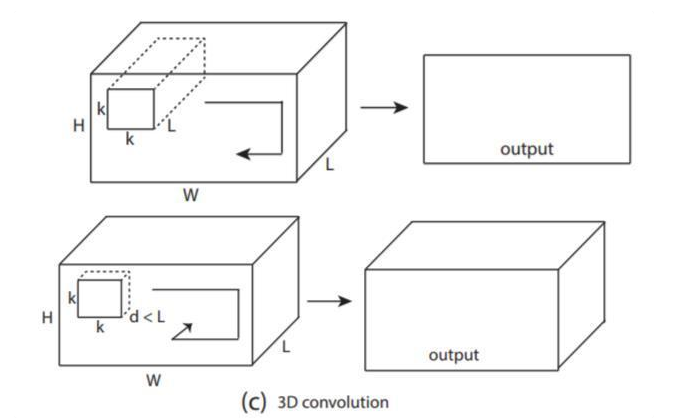
\includegraphics[width=0.66\textwidth]{DPLandCV20191224003.png}
\caption{图 3:2D CNN vs. 3D CNN [47]}
\label{DPLandCV20191224003}
\end{figure}


因此, 3D CNN 的计算复杂度随着分辨率呈现三次方增长。相比于 2D 图像处理, 3D CV 更难, 因为增加的维度使得不确定性也随之增加, 如遮挡和不同的摄像头角度(见图 4)。
下一节将涉及处理多种 3D 数据表征的解决方案, 这些方法具备新架构和预处理步骤, 专用于解决上述挑战。
%%%%%%%%%%%%%%%%%%%%%%%%%%%%%%%%%%%%%%%%%%
\section{几何深度学习}
几何深度学习(GDL)将深度学习技术扩展到 3D 数据。3D 数据的表征方式多种多样, 总体上可分为欧几里得和非欧几里得。3D 欧几里得结构化数据具备底层网格结构, 允许全局参数化, 此外, 它还具备和 2D 图像相同的坐标系统。这使得现有的 2D 深度学习范式和 2D CNN 可应用于 3D 数据。3D 欧几里得数据更适合通过基于体素的方法分析简单的刚性物体, 如椅子、飞机等。另一方面, 3D 非欧几里得数据不具备网格数组结构, 即不允许全局参数化。因此, 将经典深度学习技术扩展到此类表征是非常难的任务, 近期 [52] 提出的 Pointnet 解决了这个难题。
对目标识别有用的连续形状信息常常在转换为体素表征的过程中丢失。使用传统 CV 算法, [53] 提出可应用于体素 CNN(voxel CNN)的一维特征。这种基于平均曲率的新型旋转不变特征提升了体素 CNN 的形状识别性能。该方法应用到当前最优的体素 CNN Octnet 架构时取得了极大成功, 它在 ModelNet10 数据集上取得了 1\% 的整体准确率提升。

SLAM

视觉 SLAM 是 SLAM 的子集, 它使用视觉系统(而非激光雷达)登记场景中的路标。视觉 SLAM 具备摄影测量的优势(丰富的视觉数据、低成本、轻量级和低能耗), 且没有后处理通常需要的繁重计算工作负载。视觉 SLAM 包含环境感知、数据匹配、运动估计、位置更新和新路标登记等步骤。
对在不同条件(如 3D 旋转、缩放、光照)中出现的视觉对象建模, 以及使用强大的迁移学习技术扩展表征以实现 zero/one shot learning, 是一道难题。特征提取和数据表征方法可以有效地减少机器学习模型所需的训练样本数量。
图像定位中常使用一种两步方法:位置识别+姿势估计。前者使用词袋方法, 通过累积局部图像描述子(如 SIFT)来计算每个图像的全局描述子。每个全局描述子均被存储在数据库中, 一同存储的还有生成 3D 点云基准图的摄像头姿势。从 query 图像中提取出类似的全局描述子, 数据库中最接近的全局描述子可以通过高效搜索检索出来。最接近全局描述子的摄像头姿势可以帮助我们对 query 图像进行粗略定位。在姿势估计中, 使用 Perspective-n-Point (PnP) [13] 和几何验证等算法更准确地计算 query 图像的确切姿势。
基于图像的位置识别的成功很大程度上归功于提取图像特征描述子的能力。不幸的是, 在对激光雷达扫描图像执行局部特征提取时, 没有性能堪比 SIFT 的算法。3D 场景由 3D 点和数据库图像构成。一种方法是将每个 3D 点与一组 SIFT 描述子结合起来, 描述子对应该点被三角化的图像特征。然后将这些描述子平均为一个 SIFT 描述子, 来描述该点的外观。
另一种方法基于 RGB-D 数据构建多模态特征, 而不是深度处理。至于深度处理部分, 研究者采用基于表面法线的着色方法, 因为它对多种任务有效且具备稳健性。另一种使用传统 CV 技术的替代方法提出基于图的层级描述子 Force Histogram Decomposition (FHD), 它可以定义对象的成对结构化子部分之间的空间关系和形状信息。该学习步骤的优势是与传统词袋框架兼容, 从而出现结合了结构特征和局部特征的混合表征。

360 度摄像头

由于球面摄像头的成像特点, 每张图像都能够捕捉到 360 度全景场景, 消除了对转向选择的限制。球面图像面临的一个主要挑战是超广角鱼眼镜头导致的严重桶形畸变, 这增加了受传统人类视觉启发的车道检测和轨迹追踪等方法的实现复杂度。这通常需要额外的预处理步骤, 如先验校准(prior calibration)和 deworming。[60] 提出的一种替代方法将导航看作分类问题, 从而绕过了预处理步骤, 该方法基于原始未校准球面图像找出最优潜在路径方向。
全景拼接是该领域的另一个开放性问题。实时拼接方法 [61] 使用一组可变形网格和最终图像, 并结合利用稳健像素着色器的输入。另一种方法 [62] 将几何推理(线和消失点)提供的准确率和深度学习技术(边和法线图)实现的更高级数据提取和模式识别结合起来, 为室内场景提取结构化数据, 并生成布局假设。在稀疏结构化场景中, 由于缺乏明显的图像特征, 基于特征的图像配准方法通常会失败。这时可使用直接的图像配准方法, 如基于相位相关的图像配准算法。[23] 研究了基于判别相关滤波器(DCF)的图像配准技术, 证明基于 DCF 的方法优于基于相位相关的方法。

数据集标注和增强

对于 CV 和深度学习的结合存在一些反驳意见, 总结为一句话就是:我们需要重新评估方法, 不管是基于规则的方法还是数据驱动方法。从信号处理的传统角度来看, 我们了解传统 CV 算法(如 SIFT 和 SURF)的运算内涵, 而深度学习无法展示这些意义, 你所需要的只是更多数据。这可以被视为巨大的前进, 但也有可能是后退。本论文提到了该争论的正反方观点, 但是如果未来的方法仅基于数据驱动, 那么研究重点应该放在更智能的数据集创建方法上。
当前研究的基础问题是:对于特殊应用的高级算法或模型, 没有足够的数据。未来, 结合自定义数据集和深度学习模型将成为很多研究论文的主题。因此研究者的输出不仅涉及算法或架构, 还包括数据集或数据收集方法。数据集标注是深度学习工作流中的主要瓶颈, 需要大量的手动标注工作。这在语义分割中尤为明显, 因为该领域需要准确标注每一个像素。[20] 讨论了很多有用的半自动流程工具, 其中一些利用了 ORB 特征、多边形变形(polygon morphing)、半自动感兴趣区域拟合等算法方法。
克服数据缺乏、减少图像分类深度学习模型过拟合现象最容易也最常见的方法是, 利用标签不变的图像变换(label-preserving transformation)人为地扩大数据集。该过程叫做数据集增强, 指基于已有数据通过剪裁、缩放或旋转等方式生成额外的训练数据。人们希望数据增强步骤需要极少的计算, 且可在深度学习训练流程中实现, 这样变换后的图像就不必存储在磁盘中了。数据增强使用的传统算法方法包括主成分分析(PCA)、噪声添加、在特征空间的样本之间进行内插或外推, 以及基于分割标注建模视觉语境周边物体。

%%%%%%%%%%%%%%%%%%%%%%%%%%%%%%%%%%%%%%%%%%
\begin{figure}[H]
\centering
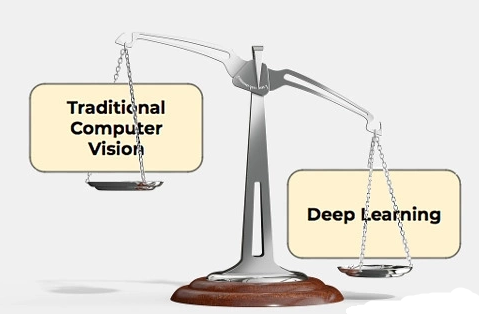
\includegraphics[width=0.66\textwidth]{tempsnip.png}
\caption{深度学习是否可以取代传统的计算机视觉}
\label{tempsnip}
\end{figure}

在进行深度学习之前, 如果你有诸如图像分类之类的任务, 这时你需要执行一个称为特征提取的步骤, 特征提取是非常“有趣的”。我这篇文章中将要提到一些传统的计算机视觉技术(包括诸如边缘检测, 角点检测, 物体检测等等)。
在使用这些技术时, 例如在特征提取和图像分类方面, 我们想的是从一类对象(例如椅子, 马等)的图像中提取尽可能多的特征, 并将这些特征视为一种“定义”(被称为“袋”)的对象。然后, 你会在其他图像中搜索这些“定义”。如果一个袋子中的大量特征位于另一个图像中, 则该图像被分类为包含该特定对象(即椅子, 马等)。
这种图像分类特征提取方法的难点在于, 你必须选择在每个给定图像中查找哪些特征。当你尝试分类的类别数量开始增加, 例如10或20时, 这会变得很麻烦并且变得几乎不可能。你是否寻找边缘?纹理信息?使用不同类型的功能可以更好地描述不同类别的对象。如果你选择使用许多特征, 则必须处理大量参数, 所有这些参数都必须由你进行微调。
那么, 深度学习介绍了端到端的学习概念, 其中(简而言之)机器被告知要针对每个特定类别的对象学习要寻找什么。它为每个对象提供了最具描述性和显着的特征。换句话说, 神经网络已经被告知发现图像类别中的底层模式。
因此, 通过端到端的学习, 你不再需要手动决定使用传统计算机视觉技术来描述你的特征。有线杂志这样说道:
例如, 如果你想教一个神经网络来识别一只猫, 那么你不要告诉它寻找胡须, 耳朵, 毛皮和眼睛。你只需要展示成千上万张猫的照片, 最终就能解决问题。如果它将狐狸误分类为猫, 你不需要重写代码, 你只需要做的是继续训练。
下面的图片描绘了特征提取(使用传统的方法)和端到端学习之间的差异:
%%%%%%%%%%%%%%%%%%%%%%%%%%%%%%%%%%%%%%%%%%
\begin{figure}[H]
\centering
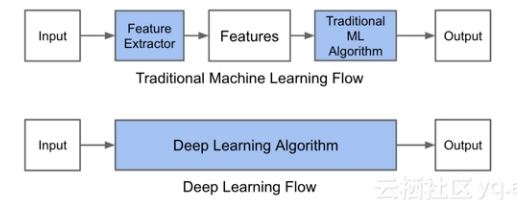
\includegraphics[width=0.66\textwidth]{DEEPlearningFlow.JPG}
\caption{特征提取和端到端学习之间的差异}
\label{DEEPlearningFlow}
\end{figure}
所以, 这是整篇文章的背景。接下来, 让我们来看看为什么传统的计算机视觉仍然是必要的, 有益的。深度学习需要大数据
首先, 深度学习需要数据, 很多很多的数据。上面提到的那些著名的图像分类模型都是在大数据集上进行训练的, 这些用于训练的数据集的前三名是:

ImageNet——包含 1000个对象类别/类的 150万个图像。
上下文中的Microsoft通用对象(COCO)——250万个图像, 91个对象类别。
PASCAL VOC数据集 ——500K图像, 20个对象类别。

比一般图像分类更容易的任务不需要这么多的数据, 但你仍然需要很多数据。如果你无法获得那么多的数据, 你根本不知道会发生什么?(确实也有一些技巧可以提高你的训练数据量, 但这些是人为的方法)。
没有充足的数据, 训练出来的模型一般表现都不好, 因为一台机器没有洞察能力, 它不能在没有看到数据的情况下概括它看到的东西。
对于你来说, 看到训练好的模型并且手动调整一些东西太困难了, 因为深度学习模型里面有数百万个参数, 其中每个参数在训练过程中都会被调整。从某种意义上说, 深度学习模式是一个黑匣子。
传统的计算机视觉为你提供了充分的透明度, 使你能够更好地评估和判断你的解决方案是否可以在训练环境之外进行工作。你可以深入了解算法中存在的问题, 如果有任何不妥, 你可以很容易地弄清楚在哪里以及需要调整什么。深度学习有时会发生过度拟合:
这可能是我支持传统计算机视觉技术研究的最佳理由。训练深度神经网络需要很长时间, 你需要专用硬件(例如, 高性能GPU), 在很长的时间内训练最新的最先进的图像分类模型。
此外, 如果你的训练模型表现不佳, 会发生什么?你必须返回并用不同的训练参数重做整个过程, 而且这个过程有时可能重复数百次。
但有时候这些都是不必要的, 因为有时传统的CV技术可以比DL更有效地解决问题, 并且代码行数更少。例如, 我曾经参与过一个项目, 以检测通过传送带的每个锡罐是否有红色的勺子。现在, 你可以训练一个深度神经网络来检测勺子, 或者你可以对红色上编写简单的颜色阈值算法(红色的某个范围内的任何像素都是白色的, 每个其他像素是黑色的), 然后计算你有多少白色像素。
了解传统的计算机视觉可能会为你节省大量时间和减少一些不必要的麻烦。传统的计算机视觉将提高你的深度学习技能:
理解传统的计算机视觉实际上可以帮助你更好地进行深度学习。
例如, 计算机视觉中使用的最常见的神经网络是卷积神经网络。但什么是卷积?它实际上是一种广泛使用的图像处理技术(例如参见Sobel边缘检测)。了解这可以帮助你了解你的神经网络做了什么, 因此可以更好地设计和调整你尝试解决的任务。
然后还有一件事叫做预处理。这是经常对你提供的模型的数据进行准备以进行训练。这些预处理步骤主要通过传统的计算机视觉技术来完成。例如, 如果你没有足够的训练数据, 则可以执行称为数据增加的任务。数据增加可以包括对训练集中的图像执行随机旋转, 移位, 剪切等, 以创建“新”图像。通过执行这些计算机视觉操作, 你可以大大增加你拥有的训练数据量。结论:
在这篇文章中, 我解释了为什么深度学习没有取代传统的计算机视觉技术, 为什么后者仍应该学习。首先, 我发现了DL经常需要大量数据才能执行的问题。其次, 深度学习对于特定任务来说可能会出现过度拟合现象。在这样的任务中, 标准的计算机视觉可以比DL更有效地解决问题, 并且代码行数更少。第三, 认识传统的计算机视觉实际上可以让你更好地进行深度学习。这是因为你可以更好地了解DL到底正在做什么, 并且你可以执行某些预处理步骤来改善DL结果。
简而言之, 深度学习只是计算机视觉的工具, 当然不是万能药。不要只用它, 因为它现在是新潮。传统的计算机视觉技术仍然非常有用, 知道它们可以为你节省时间和解决许多麻烦。
本文由阿里云云栖社区组织翻译。
文章原标题《Why Deep Learning Has Not Superseded Traditional Computer Vision》
作者:Zbigniew

北京大学信息科学技术学院教授黄铁军, 则基于自己的最新研究成果, 带来了主题为《视达(vidar):视觉新模型与超级视觉》的报告。


北京大学信息科学技术学院教授黄铁军先提出了一个问题:人为什么躲不过子弹?原因是:人的眼睛往大脑传送神经脉冲的速度比较慢, 而且每秒只能传几十个脉冲, 所以, 当一颗子弹飞过来时, 眼睛根本来不及向大脑传输信号。
基于此, 他较为尖锐地指出, 现在 90\% 做计算机视觉的研究者根本还没搞明白视觉到底是什么, 因而现在用摄像头采集视频+算法的技术研究路线和思维方式从根本上来说都是错误的。并且, 用视频作为视觉信息的表达方式的这一起点, 就是错的。
视频实际上是影视产业发展的产物, 它利用的其实就是人类视觉系统的缺陷——视觉暂留, 来给人类以连续的画面感, 而生物视觉则是视网膜接收连续的光子撞击, 再由神经节细胞接收到足够刺激后发放脉冲, 接着脉冲序列被传送给大脑, 最后大脑从脉冲序列中解码出外部世界,
因此, 要真正实现机器智能, 就必须放弃视频这一概念, 用新的思路去做研究:了解从眼睛到大脑的神经脉冲是如何编码外界的视觉信息的。基于这一思路, 黄铁军教授在视觉信息处理方面最近开展了一个工作, 便是模仿从视网膜到大脑的神经脉冲对外界视觉信息进行编码。他将这项工作称之为视达(vidar)。

计算机视觉的研究者应该彻底改变用摄像头+算法的研究思路:

第一, 不再用以前的识别摄像机, 而要用新的视达芯片和摄像机来抓识取过程;

第二, 不要在计算机上编算法, 而要在脉冲神经网络做脉冲序列。

山世光研究员指出, 随着人脸识别已经取得了非常大的进展, 接下来将会从「看脸」时代转向「读心」的时代, 从依赖强大的数据的学习算法转向弱监督小规模数据驱动的视觉学习算法。因此, 打造有温度、有温情的 AI 系统, 非常重要。

对于「读心」, 他认为可以从三个层次来开展工作:

第一, 测量生理性特征, 比如身高、体重、心率、呼吸、血压、血氧、眨眼率、视线、瞳孔缩放、皮肤状况、醉酒状态等等。

第二, 评估心理状态。表情很多时候是虚假的, 而微表情则更能体现人试图隐藏的内心情绪。这些心理状态的评估可以应用到学习、驾驶、健康等方面。

第三, 通过观察生理特征和心理状态, 来评估人的内心精神状况, 包括是否抑郁、幸福等精神层面的辅助诊断。

然而在具体的技术实现上, 「读心」首先就面临着是数据稀缺的挑战, 比如针对自闭症儿童的数据, 有个几十人就已经算多的了。那么如何在非常小规模的数据环境下做好机器学习呢?

可以从以下三个方向来克服这个挑战:

第一, 自监督学习, 思路是针对小样本, 尽可能地采用借鉴人的注意机制的方法, 找到最值得关注的区域并提取特征, 从而即便在小样本情况下也可以实现比较好的视觉特征学习。

第二, 弱监督学习, 思路是通过引入不同的任务, 进行多个任务的协同处理, 从而将不同任务的算法进行优势互补, 实现弱监督条件下的学习。

第三, 半监督学习, 思路是协同训练一部分带标签的数据和另一部分没有标签的数据, 让二者同时学习多个模型, 互相补充和支持, 将这些没有标签的数据也用起来。

未来十年, AI 会深刻地改变各行各业, AI 算法也会越来越深刻地了解人类, 然而现有的算法还不足以支撑社会各界对 AI 的预期。如何在数据稀缺情况下做机器学习是未来要克服的挑战之一, 他今天分享的仅仅是实现标签从无到有、由弱变强、从小到大的思路, 而其他的思路, 例如如何将领域知识设计成一种通用的算法等, 也是值得领域研究者关注和研究的方向。

%%%%%%%%%%%%%%%%%%%%%%%%%%%%%%%%%%%%%%%%%%%%%%%%%%
\section{作 业 }
%%%%%%%%%%%%%%%%%%%%%%%%%%%%%%%%%%%%%%%%%%%%%%%%
\begin{custom}[explorecolor]{探索}

\end{custom}

%%%%%%---------------------------------
\begin{think}
  
\end{think}